\NeedsTeXFormat{LaTeX2e}

% Rahmenumgebung f�r Studien Diplomarbeiten
% Erstellt von Oomke Weikert und Florian Keiler
% �nderungen im file _changelog.txt

% Titel und Autor der Arbeit unten im 
% \hypersetup Kommando �ndern
% ...und nat�rlich auf der Titelseite (title.tex bzw. title_en.tex)

% um pdf-file zu erzeugen:
% compilieren mit:
% pdflatex 
% bibtex
% pdflatex  
% pdflatex 
% (Hinweis: Das pdf-file darf bei Aufruf von pdflatex
% nicht im Adobe Reader ge�ffnet sein. Wenn man das
% pdf-file mit Ghostview �ffnet, muss es nicht geschlossen
% werden, und man kann dort die gerade bearbeitete Seite
% offen lassen)

% Im figures Ordner m�ssen die Bilder z.B. in pdf oder jpg Format liegen,
% mit pdflatex k�nnen *keine* eps Bilder benutzt werden.
% Das pdf file darf beim Kompilieren nicht 
% im Acrobat Reader ge�ffnet sein!!!

% um ps-file zu erzeugen:
% compilieren mit:
% latex 
% bibtex
% latex 
% latex 
% dvips

% dvips Aufruf f�r Type-1 Schriften: 
% dvips -t a4 -Ppdf 
% (alte GhostScript-Version: dvips -t a4 -Ppdf -G0) 
% Umwandeln in pdf mit Acrobat Distiller 
% oder mit ps2pdf (in GhostScript enthalten)


\documentclass[a4paper, twoside, 12pt, openright]{report}

\newif\ifmakeindex
\makeindextrue % generate index
%\makeindexfalse % don't generate index

\ifmakeindex
% fuer Stichwortverzeichnis
\usepackage{makeidx}

% Stichwortverzeichnis erstellen
\makeindex
\fi


\newif\ifenglish
\englishtrue   % english document
%\englishfalse  % german document

\usepackage[margin=1cm,format=hang,font=small,labelfont=bf,textfont=sl]{caption}
% angepasste Bildunterschriften
% Doku siehe beigef�gtes pdf-file

% subfig is here
\usepackage{subfig}

\usepackage[english]{babel}

\usepackage[latin1]{inputenc}
% Unterstuetzen von deutschen Umlauten

\usepackage{t1enc}
% Verwenden von DC-Fonts (erlaubt richtiges Trennen
% auch in Worten mit Umlauten)

%\usepackage{times} 
  % Saves a lot of ouptut space in PDF...
  % ..after conversion with ps2pdf or Adobe Distiller	 
	% �ndert aber die Schriftart! (Times statt computer modern roman)
\usepackage{courier} % fett *und* typewriter nur damit m�glich?
% �ndert normale Schrift nicht!

\usepackage{cite}
% Automatisches Zusammenfassen von Literaturstellen

\usepackage{fancyheadings}	
%STY-file fancyheadings.sty nicht standardm��ig in miktex enthalten
%evtl. durch fancyhdr ersetzen

\usepackage{float}
%This package improves the interface for defining floating objects such
%as figures and tables in LaTeX.  It adds the notion of a `float style'
%that governs appearance of floats.  New kinds of floats may be defined
%using a \newfloat command analogous to \newtheorem.  This style option
%also incorporates the functionality of David Carlisle's style option
%`here', giving floating environments a [H] option which means `PUT IT
%HERE' (as opposed to the standard [h] option which means `You may put
%it here if you like').

\usepackage{verbatim}		
%This package reimplements the L A T E X verbatim and verbatim* envi- 
%ronments. In addition it provides a comment environment that skips any 
%commands or text between \begin{comment} and the next \end{comment}. 
%It also defines the command verbatiminput to input a whole file verbatim. 

\usepackage{amsmath}

%\usepackage{rotating}

\usepackage{array}
% wird benutzt von macro.tex f�r \Case

\usepackage{ifthen}
% wird benutzt von macro.tex \ifthenelse

\usepackage{longtable}
% f�r lange Tabellen gr��er als eine Seite mit \begin{longtable} .. \end{longtable}

\usepackage{varioref}
% Kommando \vref verweist mit Seitenzahl

\usepackage{readfile}
% ASCII-File einbinden mit
% \readit{fftdb.m}{\tt} 
% 2. Argument (\tt) gibt zu benutzende Schriftart an 
\usepackage{shapepar}
\usepackage{setspace}
\usepackage{colortbl}
\usepackage{color}
\usepackage{xcolor} 
%\usepackage{caption} %added by fu


\usepackage{listings}

\lstloadlanguages{}

\lstloadlanguages{C,C++,Java,Matlab,HTML,TeX,XML}

\definecolor{mygreen}{RGB}{28,172,0} % color values Red, Green, Blue
\definecolor{mylilas}{RGB}{170,55,241}
\definecolor{theme_color}{HTML}{C50042}


%\usepackage{subcaption}
%\lstset{}% restore default
%# title={Titel}:  gibt einen Titel zur Umgebung an (erscheint �ber dem Code zentriert)
%# caption={Titel}:  
%# label=Name:

\lstset{
				frame=lines, %Umrandung (single|none|shadowbox|lines|bottomline|topline|leftline)
				framerule=1pt, %Rahmenbreite
				tabsize=4, %Anzahl der Zeichen f�r ein TAB
				backgroundcolor=\color{lightgray}, %Hintergrundfarbe
				emph={}, %hebt die angegebenen W�rter hervor
				emphstyle=\underbar, %unterstreicht hervorgehobene W�rter
				columns=fixed, %Zeichenabstand (fixed | flexible | fullflexible)
				lineskip=0pt, %Zeilenabstand
				basicstyle=\ttfamily,%\ttfamily,
				% identifierstyle=\color{black},
    %     commentstyle=\color{darkgreen},
    %     stringstyle=\color{viola},
    %     keywordstyle=\color{darkblue},
				% ndkeywordstyle=\color{black},
				% showspaces=false,
				% showtabs=false,
				% numbers=none, %Zeilennummern (none|left|right)
				% %numbertype=\ttfamily,
				% breaklines=true,
    %     captionpos=b,
    %     extendedchars=false
    language=Matlab,%
    %basicstyle=\ttfamily\fontsize{8}{5}\selectfont,
    breaklines=true,%
    morekeywords={matlab2tikz},
    keywordstyle=\color{blue},%
    morekeywords=[2]{1}, keywordstyle=[2]{\color{black}},
    identifierstyle=\color{black},%
    stringstyle=\color{mylilas},
    commentstyle=\color{mygreen},%
    showstringspaces=false,%without this there will be a symbol in the places where there is a space
    %numbers=left,%
    %numberstyle={\tiny \color{black}},% size of the numbers
    %numbersep=9pt, % this defines how far the numbers are from the text
    %emph=[1]{for,end,break},emphstyle=[1]\color{red}, %some words to emphasise
    %emph=[2]{word1,word2}, emphstyle=[2]{style},  
}

%\usepackage{fancybox}
%\usepackage{theorem}
%\usepackage{amsbsy}
%\usepackage{nomencl}        % unterst�tzt Symbolverzeichnisse
%\usepackage{makeidx}
%\usepackage{multind}

\def\boxes{yes}
% \boxes == yes makes boxes around desired formulas by \Mbox
% wird benutzt von macros.tex
 

% pdf-tex settings:
% ------------------------
% detect automatically if run by latex or pdflatex

\usepackage{tikz}
\usetikzlibrary{arrows,calc,positioning,shapes}
\tikzset{
axis/.style={<->},
}
\usepackage{pgfplots}
\pgfplotsset{compat=1.5}
\newlength\figureheight 
\newlength\figurewidth 

\usepackage{bm}
\usepackage{amsfonts}
\usepackage{amsmath}
\usepackage{amssymb} %added by fu
\usepackage{textcomp} %added by fu

%\usepackage{array} %added by fu
\usepackage{natbib}
\usepackage{setspace} %added by fu
%\usepackage{tabu}
\usepackage{tabularx}
%\usepackage{multirow} %added by fu
%\usepackage{graphicx}
%\usepackage{subcaption} %added by fu
\usepackage{mathtools}
%\usepackage{wrapfig}
\usepackage{longtable}
\DeclareMathOperator*{\argmax}{arg\,max}
% small math characters
\newcommand{\sml}[1]{\mbox{\scriptsize $#1$}}
\DeclarePairedDelimiter\abs{\lvert}{\rvert}%
\DeclarePairedDelimiter\norm{\lVert}{\rVert}
\usetikzlibrary{pgfplots.groupplots}
\usepgfplotslibrary{external} % make tikz compile only once
							  % added by fu
\tikzexternalize
%\usepgfplotslibrary{pggroupplots} % use group plots
\newcommand{\specialcell}[2][c]{%
  \begin{tabular}[#1]{@{}c@{}}#2\end{tabular}} %added by fu
  											   % for new lines in table cell

\newcommand{\cellpadding}[1]{%
  \vspace{-5pt} \\#1 \vspace{5pt}} %added by fu
  											   % for new lines in table cell

%\usepackage{enumitem} %for better itemize
%\setlist{itemsep=8pt}

%
% this makes list spacing much better.
%
\newenvironment{my_enumerate}{
\begin{enumerate}
  \setlength{\itemsep}{1pt}}{\end{enumerate}
}

\usepackage{ifpdf}
%\newif\ifpdf  
%\ifx\pdfoutput\undefined
%   \pdffalse
%\else
%   \pdfoutput=1
%   \pdftrue
%\fi

\ifpdf % compiling with pdflatex
   %\usepackage[pdftex]{graphicx}    %%%%%%%%%%%%%%comment out by fu
   %\DeclareGraphicsExtensions{.pdf, .png, .jpg, .tikz} %%%%%%%%%%%%%%%%%comment out by fu
   \usepackage[pdftex,
	bookmarks,
	%colorlinks=false, % instead of colors, now boxes are used for links
	colorlinks=true,
	urlcolor=black, %blue,
	linkcolor=black, %red, %normal internal links
	citecolor=black, %green, %citation links
	%pagebackref, %link from references back to page of citation
	linktocpage, 
	% im Inhaltsverzeichnis Link auf Seitenzahl (sonst Probleme bei langen Zeilen)
	%breaklinks = true, % f�r Links l�nger als 1 Zeile
	%hypertexnames = false,  % f�r Links zu Figures?
	bookmarksopen, %open all bookmark folders
	bookmarksnumbered, %use section numbers with bookmarks
    pdfpagemode=UseOutlines, %show bookmarks
	% http://www.tex.ac.uk/cgi-bin/texfaq2html?label=pdfpagelabels
	plainpages=false, % eigene Seitenanker f�r r�mische/arabische Seitenzahlen
	pdfpagelabels, % im Abode Reader Seitenzahl als z.B. "iii (3 von 20)" anzeigen
%	pdfstartview=FitH
	pdfstartview=FitV
	]{hyperref}
    \pdfadjustspacing=1                %%% force LaTeX-like character spacing
    \pdfcompresslevel=9
	\pdfcatalog{                 
	% Catalog dictionary of PDF output. 
    % /PageMode /UseNone          
    % /URI (http://www.fi.muni.cz/)
	%       
	% pdfscreen-like setting might look like:
	%     /PageMode /none 
	%     /ViewerPreferences << 
	%         /HideToolbar true            
	%         /HideMenubar true 
	%         /HideWindowUI true 
	%         /FitWindow true 
	%         /CenterWindow true 
	%	
	% /PageMode determines how Acrobat displays the document on startup. 
	% The possibilities for the latter are explained below:
	% Supported /PageMode values.
	% /UseNone 		neither outline nor thumbnails visible
	% /UseOutlines 	outline visible
	% /UseThumbs 	thumbnails visible
	% /FullScreen 	full--screen mode
	% In full--screen mode, there is no menu bar, window controls, 
	% nor any other window present. The default setting is /UseNone.
	} %end of \pdfcatalog
\else % compiling with latex
 \usepackage[dvips]{graphicx}
%  \usepackage{color}
  \DeclareGraphicsExtensions{.eps}
  \usepackage[
    dvips,
%	ps2pdf,  % statt dvips, Unterschied???
	bookmarks,
  	colorlinks=false,  % for final paper without colors
%  	colorlinks=true,
	linktocpage, 	
	% im Inhaltsverzeichnis Link auf Seitenzahl (sonst Probleme bei langen Zeilen)
	%breaklinks = true, % f�r Links l�nger als 1 Zeile
	% funktioniert *nicht* korrekt f�r lange Zeilen mit gs < 7.05.3 ?
%	pdfstartview=FitH, % funktionfor different stakeholders of prostate cancer, e.g., patients, doctors and pharmaceutical companies.iert NICHT mit Adobe Distiller
	bookmarksopen, %open all bookmark folders
	bookmarksnumbered, %use section numbers with bookmarks
    pdfpagemode=UseOutlines, %show bookmarks
	pdfstartview=FitV
   ]{hyperref}
  % hyperrefs are active is the pdf file after conversion
  \hypersetup{
	pdfcreator  = {LaTeX with hyperref package},
	pdfproducer = {dvips + ps2pdf}
  }
\fi

% CHANGE TITLE AND AUTHOR !!!
\hypersetup{
  pdftitle={Studien/Diplomarbeit},
	pdfauthor={Autor},
	pdfsubject  = {Studien/Diplomarbeit, UniBwH, Professur ANT, \today},
	pdfkeywords = {}
}

% ------------------------


%Breite der Bild/Tabellenbeschriftungen:
%\setlength{\LTcapwidth}{\captionwidth}

%Schriftgr��e/Zeilenvorschub in Tabellen:
\def\tablefontsize{\normalsize}
\def\tablespacing{1.0} % linespacing in tables
  
\newcommand{\bc}{\begin{center}}
\newcommand{\ec}{\end{center}} 

\newcommand{\be}{\begin{equation}}
\newcommand{\ee}{\end{equation}} 
\newcommand{\bea}{\begin{eqnarray}}
\newcommand{\eea}{\end{eqnarray}}

\newcommand{\bi}{\begin{itemize}}
\newcommand{\ei}{\end{itemize}}

\newcommand{\bmp}{\begin{minipage}[c]{\columnwidth} \bc}
% argument: vertical position: c, t, b
\newcommand{\emp}{\ec \end{minipage} }

\newcommand{\beg}{\hspace{0.5cm}\begin{minipage}{14cm}}
\newcommand{\eeg}{\end{minipage}\vspace{1cm}}


%%%%%%%%%%%%%% tables %%%%%%%%%%%%%%%%%%%%%%%
\newcommand{\bt}[1]
% #1: table placing: htbp
    {    \begin{table}[#1] %htbp 
         \begin{center}
         \renewcommand{\baselinestretch}{\tablespacing}
         \tablefontsize
    }

%Tabelle mit gr��erem Zeilenvorschub:
\newcommand{\btline}[2]
% #1: table placing: htbp
% #2: linespacing in table, e.g. 1.4
{   \def\tablespacing{#2}
    \bt{#1}
} 

\newcommand {\et}[2] 
% #1: caption
% #2: label without 'tab:'
    {
     \caption{#1.} 
     \label{tab:#2}
     \end{center} 
     \end{table}
     \def\tablespacing{1.0} 
    % reset linespacing for next table
}

\newcommand {\btab}{\begin{tabular}}
\newcommand {\etab} {\end{tabular}}

\newcommand{\mc}{\multicolumn}
\newcommand{\mr}{\multirow}

% columns in math mode:
\newcolumntype{C}{>{$}c<{$}}
\newcolumntype{L}{>{$}l<{$}}
\newcolumntype{R}{>{$}r<{$}}

\newcommand{\pbs}[1]{\let\temp=\\#1\let\\=\temp}
%preserve backslash, s. companion, p108



%%%%%%%%%%%%%% figures %%%%%%%%%%%%%%%%%%%%%%%
\newcommand{\fig}[4]{
% Bild mit 80% der Seitenbreite
% arguments:	
% #1: file without extension eps
% #2: caption
% #3: label
% #4: placing of the figure: e.g. htbp
\begin{figure}[#4]			      
\begin{center}
   \includegraphics[width=.8\columnwidth]{figures/#1}
   \caption{#2.}
   \label{fig:#3}
\end{center}
\end{figure}
}

\newcommand{\figscale}[5]{
% arguments:	
% #1: file without extension eps
% #2: caption
% #3: label
% #4: placing of the figure: e.g. htbp
% #5: width of figure
\begin{figure}[#4]			      
\begin{center}
   \includegraphics[width=#5\columnwidth]{figures/#1}
   \caption{#2.}
   \label{fig:#3}
\end{center}
\end{figure}
}

\newcommand{\figscaletwo}[6]{
% arguments:	
% #1: file1 without extension eps
% #2: file2 without extension eps
% #3: caption
% #4: label
% #5: placing of the figure: e.g. htbp
% #6: width of figure
\begin{figure}[#5]			      
\begin{center}
   \includegraphics[width=#6\columnwidth]{figures/#1}~\\
   \includegraphics[width=#6\columnwidth]{figures/#2}
   \caption{#3.}
   \label{fig:#4}
\end{center}
\end{figure}
}

\newcommand{\figtwo}[5]{
% two figures labeled (a) and (b) side by side
% arguments:	
% #1: file1 without extension eps
% #2: file2 without extension eps
% #3: caption without fullstop
% #4: label
% #5: placing of the figure: e.g. htbp
\begin{figure}[#5]			      
\begin{center}
    \btab{cc} 
   \includegraphics[width=0.45\columnwidth]{figures/#1}
    &	 
   \includegraphics[width=0.45\columnwidth]{figures/#2}
    (a)&(b)
    \etab 
	\caption{#3.}
	\label{fig:#4}
\end{center}
\end{figure}
}

\newcommand{\figTwo}[6]{
% two figures labeled (a) and (b) on top/bottom
% arguments:	
% #1: file1 without extension eps
% #2: file2 without extension eps
% #3: caption without fullstop
% #4: label
% #5: placing of the figure: e.g. htbp
% #6: width of figures as ratio, e.g. 0.7
\begin{figure}[#5]			      
\begin{center}
   \includegraphics[width=#6\columnwidth]{figures/#1}
(a)\\
\vspace{1 em}
   \includegraphics[width=#6\columnwidth]{figures/#2}
    (b)\\
    \caption{#3.}
    \label{fig:#4}
\end{center}
\end{figure}
}

%%%%%%%%%%%%%%%%%%%%%%%%%%%%%%%%%%%%%%%%%%%%%%

\newcommand{\C}[1]{\texttt{#1}} %Typewriter-Font
\newcommand{\tild}{\~~\hspace{-1 ex}} %Tilde ~

\newcommand{\equi}{\Leftrightarrow} %�quivalenz <=>
\newcommand{\concl}{\Rightarrow}    %daraus folgt =>
%Matrix:
\newcommand{\matr}[2]{\left ( \begin{array}{#1} #2 \end{array} \right )}
% #1 alignment of colums, e.g. ccc
% #2 contents of matrix
%Vektor:
\newcommand{\vect}[1]{\left ( \begin{array}{c} #1 \end{array} \right )}
%Fettschrift im Mathemodus:
\newcommand{\mbf}[1]{\mathbf{#1}} %boldface
\newcommand{\gbf}[1]{\boldsymbol{#1}} %boldface greek letters
%Verweis auf Gleichungen mit Klammern um Gl.-Nr.
%\newcommand{\eqref}[1]{(\ref{#1})}
% \eqref defined in package amsmath


\newcommand{\freqorig}{\ensuremath{\circ\hspace{-.1em}\mbox{---}\!\bullet}}
\newcommand{\freq}{\mbox{~}{\circ\hspace{-.1em}\mbox{---}\!\bullet}\mbox{~}}
	% correspondence symbol time<->freq 
\newcommand{\freqswap}{\ensuremath{\bullet\!\mbox{---}\hspace{-.1em}\circ}}
\newcommand{\freqv}{\begin{turn}{90} \freqswap \end{turn}}
	% vertical correspondence symbol
	% time 
	% freq
\newcommand{\timeh}{\mbox{~}{\bullet\!\mbox{---}\hspace{-.1em}\circ}\mbox{~}}
	% correspondence symbol freq<->time
\newcommand{\timev}{\begin{turn}{90} \freqorig \end{turn}}
	% vertical correspondence symbol
	% freq
	% time

\newcommand{\Case}[1]{\left\{ \begin{array}{ll} #1
    \end{array}\right. } 


\newcommand{\Mbox}[1]{
\ifthenelse{\equal{\boxes}{yes}}
{%\ensuremath
\fbox{$\displaystyle #1$}}
{#1}}

%box around a equationarray
%argument is the contents of the eqnarray environment
\newcommand{\Mboxarray}[1]{
\ifthenelse{\equal{\boxes}{yes}}
{\bc\fbox{\begin{Beqnarray} #1 \end{Beqnarray}}\ec}
{\bea #1 \eea}
}


\newcommand{\suml}{\sum\limits}
% limits of sum UNDER the sign instead of beside it, e.g. in fractions

\newcommand{\intl}{\int\limits}
% limits of int UNDER the sign instead of beside it


\newcommand{\logd}{\mbox{ld\,}} %base 2 logarithm

\newcommand{\erw}[1]{E\left\{#1\right\}} %Erwartungswert


% make ',' an ordinary Symbol in decimal numbers
% Unterdr�ckung des Zwischenraums hinter einem Komma (z.B. in Dezimalzahlen)
% Steht im Mathemodus hinter dem Komma ein Leerzeichen, wird es als Trennzeichen
% (mit Zwischenraum) benutzt, sonst als Dezimalkomma.
 \mathchardef\CommaOrdinary="013B
 \mathchardef\CommaPunct   ="613B
 \mathcode`,="8000   % , im Math-Mode aktiv ("8000) machen
 {\catcode`\,=\active
  \gdef ,{\obeyspaces\futurelet\next\CommaCheck}}
 \def\CommaCheck{\if\space\next\CommaPunct\else\CommaOrdinary\fi}

% define the size of the region where text can appear on the page
\setlength{\hoffset}{-1in}
\textwidth 15.7cm
\textheight 24cm %24.4cm
\topmargin -1cm %-1.6cm
\oddsidemargin 2.7cm
\evensidemargin 2.6cm
%\oddsidemargin -3cm
%\evensidemargin -3cm
\headheight 15pt%[12]
\headsep 1.2cm%[25pt]
%\setlength{\footheight}{15pt} %[12]
%\columnsep 0.8cm

% setzt den Einzug bei neuem Absatz zu null
\setlength{\parindent}{0pt}
% oder \parindent0cm

%Abstand vor neuem Absatz
%wird in abstract.tex benutzt
\def\parspacing{2.5ex}
\setlength{\parskip}{\parspacing} 

% enable following command if you don't want extra space after points
\frenchspacing

\renewcommand{\textfraction}{0.1}
% Mindestanteil an Text auf einer Seite, 
% in Prozent, default: 0.2
 
\renewcommand{\topfraction}{1}
% Maximaler Anteil der von Gleitobjekten am Kopf der Seite 
% eingenommen werden kann, in Prozent, default: 0.7

\setcounter{topnumber}{10} 
% number of float objects at top of page, default: 2

\setcounter{totalnumber}{10} 
% number of float objects on one page, default: 3


\setcounter{secnumdepth}{3}
% depth of numbering, see companion p.20-21
% for report:   chapter: 0, section: 1, subsection: 2
%       subsubsection:3,paragraph: 4,   subparagraph: 5

\setcounter{tocdepth}{2}

\setlongtables
% for equal column width on different pages of a longtable, see companion, p 122
% has to be disabled to reset, only widest width is saved, 
%so there's an error, if this entry is shortened!


\addto\captionsenglish{% 
	\renewcommand{\lstlistlistingname}{List of Sourcecodes} % default: "Listings"
	\renewcommand{\lstlistingname}{Sourcecode} % default: "Listing"
}



%\makeglossary

\begin{document}
\tikzstyle{block} = [rectangle, draw, text width=6em, text centered,  minimum height=3em]
\tikzstyle{block1} = [rectangle, draw, text width=9em, text centered,  minimum height=2em]
\tikzstyle{block2} = [rectangle, draw, text width=12em, text centered,  minimum height=2em]
\onehalfspacing
\definecolor{gold}{rgb}{0.85,.66,0}
\definecolor{viola}{rgb}{0.5,0,0.5}
\definecolor{darkblue}{rgb}{0,0,.6}
\definecolor{darkred}{rgb}{.6,0,0}
\definecolor{darkgreen}{rgb}{0,.6,0}
\definecolor{red}{rgb}{.98,0,0}
\definecolor{lightgray}{rgb}{.99,.99,.97}


%HSU Corporate Design
\definecolor{hsurot}{cmyk}{0,1.00,0.43,0.185}
\definecolor{hsugrau}{cmyk}{0,0.085,0.15,0.43}
\definecolor{hsugelb}{cmyk}{0,0.15,0.60,0}
\definecolor{hsublau}{cmyk}{1.00,0.38,0,0.69}
\definecolor{hsugruen}{cmyk}{1.00,0,0.47,0.47}
\definecolor{hsuoliv}{cmyk}{0,0,1.00,0.47}
\definecolor{hsuorange}{cmyk}{0,0.43,1.00,0.18}
\definecolor{hsuhellrot}{cmyk}{0,0.76,0.83,0.11}

 

% 60%
\colorlet{hsurot60}{hsurot!60}
\colorlet{hsugrau60}{hsugrau!60}
\colorlet{hsugelb60}{hsugelb!60}
\colorlet{hsublau60}{hsublau!60}
\colorlet{hsugruen60}{hsugruen!60}
\colorlet{hsuoliv60}{hsuoliv!60}
\colorlet{hsuorange60}{hsuorange!60}
\colorlet{hsuhellrot60}{hsuhellrot!60}

% 30%
\colorlet{hsurot30}{hsurot!30}
\colorlet{hsugrau30}{hsugrau!30}
\colorlet{hsugelb30}{hsugelb!30}
\colorlet{hsublau30}{hsublau!30}
\colorlet{hsugruen30}{hsugruen!30}
\colorlet{hsuoliv30}{hsuoliv!30}
\colorlet{hsuorange30}{hsuorange!30}
\colorlet{hsuhellrot30}{hsuhellrot!30} % several predefined colors - including the HSU corporate Design.

\pagenumbering{roman} % sonst gibt es 2 mal Seiten 1 und 2 (arabisch)
% so werden Probleme bei hyperlinks vermieden

%!TEX root = thesis.tex
%\def\voff{1cm}
%\addtolength{\voffset}{-\voff}

%\vspace{-2cm}
\pdfbookmark[1]{Title page}{sec:title}  % Bookmark im pdf file
\begin{titlepage}
\label{sec:title}

%\enlargethispage{\voff}
\large 
\begin{center}

\vspace{3cm}
% Unilogo mit Link auf Webseite
% \href{http://www.tuhh.de} 
% {
% 
\includegraphics[width = .45\textwidth]{figures/tuhh_logo.png} 
% \includegraphics[width = .45\textwidth]{figures/bosch_logo.png}
% }
\begin{figure}[ht]
\centering%%% not \center
%\subfigure[Figure A]{\label{fig:a}\includegraphics[width=60mm]{example-image-a}}
\subfloat{
\includegraphics[width=.35\textwidth]{figures/tuhh_logo.png}}
\hspace{20pt}
\subfloat{\includegraphics[width=.45\textwidth]{figures/bosch_logo.png}}
\end{figure}

\vspace{2cm}

\begin{minipage}{.9\linewidth}
{\centering\Huge\bf Indoor Human Tracking based on Dynamic Models from Convolutional Neural Networks \par} 
% \par ist nötig für korrekten Zeilenabstand im Titel
\end{minipage}

\large 

%\vspace{1.5cm}
%{von\\[.3cm] {\bf \LARGE Autor}\\[1cm] 
%\huge	{ \bf \it Diplomarbeit} \\[1cm]}

\vspace{1.5cm}
{\huge{\bf \it Master Thesis} %\\[1cm]
}

\vspace{0.6cm}
{
\Large by \\[.5cm] 
{\bf \LARGE \huge Liangcheng Fu}\\[1.5cm]
}

\vfill
\begin{tabular}{ll}
Start date:& 01 August 2017\\
End date:& 30 January 2018\\
\\
First Examiner:&  Prof. Alexander Schl\"afer\\
Second Examiner:&  Prof. Dr.-Ing. habil. Udo Z\"olzer\\
Supervisor:&  Johannes D\"ollinger\\
\end{tabular}
\end{center}
\vspace{2cm}

\end{titlepage}

%\addtolength{\voffset}{\voff}

\thispagestyle{empty} % Titelr�ckseite (S. 2) ohne Seitennummer

\cleardoublepage

\newcounter{pageno}
\setcounter{pageno}{1} %titlepage = page 1, but pagenumber not printed
\addtocounter{pageno}{1}

% \cleardoublepage
% %!TEX root = project_report.tex
\pdfbookmark[1]{\abstractname}{sec:abstract}  % Bookmark im pdf file
\begin{abstract}
\label{sec:abstract}
\addtocounter{pageno}{1}
\setcounter{page}{\arabic{pageno}}
\thispagestyle{plain}
\begin{center}
\begin{minipage}[t]{\linewidth} 
\setlength{\parskip}{\parspacing}

% Inspired by cognitive science studies, Malisiewicz and his colleagues proposed ensemble of \textit{exemplar}-SVMs for object detection applications \cite{malisiewicz2011}. They reported that their algorithm  has comparable performance with other more complex methods. In this project work, further investigations on usage of \textit{exemplar}-SVMs are carried out. Precisely, \textit{exemplar}-SVMs are used for object classification in the context of maritime objects image set. Besides the Histogram of Gradients (HoG) feature used in their original work, Convolutional Neural Network (CNN) feature is also used in this project. The results show that, with linear SVM as benchmark, \textit{exemplar}-SVMs algorithm does not improve the performance in terms of classification accuracy. However, since the algorithm is able to retrieve images in the training set which have the same aspect ratio as the test image, it can be used for meta-data (e.g., segmentation and 3D model) transfer, which could be beneficial for overall scene understanding. 
\textbf{Background}: Thanks to the prevalence of Internet, nowadays many patients turn to online resources to seek information and emotional supports. Particularly, thanks to their easy access to discussion boards and chat rooms, Online Health Communities (OHCs) are more active. The posts that patients write on OHCs provide diverse and huge amount of information on patients' life. \\
\\
\textbf{Objective}: To explore how OHCs affect cancer patients' emotional state and what topics are been discussed. Moreover, investigate patients' opinions on keywords consisting of drugs, drug effects and therapies. \\
\\
\textbf{Method}: Web mining techniques are used to collect posts from OHCs and sentiment analysis with machine learning approach is applied on those posts. Besides, topic model is trained for automatically classifying posts to different topics. \\
\\
\textbf{Results}: Posts from two prostate cancer communities are collected. The first community is in English, consisting of 341,326 posts and the other one is in German with 69,089 posts. The best machine learning models achieve 81.66\% and 74.71\% accuracy for two communities respectively. The observations are : 1) For threads that start with negative sentiment, the vast majority of them (more than 92\% for both communities) have positive sentiment changes after their interactions with other community users. 2) Most of frustrating topics gain more sentiment change towards the positive side than normal and pleasant topics. 3) The average sentiment of threads containing each keyword is shown, which reflects patients' attitudes towards these drugs, drug effects and therapies. \\
\\
\textbf{Implications}:  1) Since sentiment of most negative originating threads change positively, this proves OHCs are effective to improve users' emotional state. 2) The topic model, together with machine learning model for extracting sentiment, can be used as a tool to monitor thread topic and its sentiment. The community administrator could make use of it to enhance community supports. 3) Patients' attitudes towards drugs, drug effects and therapies could be exploited by different stakeholders of prostate cancer, e.g., patients, doctors and pharmaceutical companies.   \\

\end{minipage}
\end{center}

\end{abstract}



% \cleardoublepage
% \begin{center}
\pdfbookmark[1]{Statement}{sec:statement}  % Bookmark im pdf file
{\Huge \bf Statement}
\label{sec:statement}
\end{center}
Hereby I do state that this work has been prepared by myself and with the help which is referred within
this thesis.

%Hiermit erkl�re ich, dass die vorliegende Arbeit von mir selbst�ndig und nur unter Verwendung der angegebenen Quellen und Hilfsmittel erstellt wurde.

\vspace{15cm}

Hamburg, 19. December 2016


% \cleardoublepage
% \pdfbookmark[1]{Foreword}{sec:vorwort}  % Bookmark im pdf file
\chapter*{Foreword}
\label{sec:vorwort}

I would like to use this opportunity to express my gratitude to Northern Institute of Technology Management (NIT). I spent two fabulous years with colleagues, staffs and teachers from NIT. What makes these two years so special and unforgettable is not only the excellent education, but also the international atmosphere and the friendships we developed over time.    

I am also appreciated for the help and guidance I received from Prof. Dr. Corneliue Herstatt, Prof. Dr. Christian L\"uthje and from supervisor Dipl.-Ing. Moritz G\"oldner. I am really grateful for their patience over these four months and their attitudes towards scientific researches inspired me a lot.

Special thanks to all my friends who make my study life more enjoyable. Lastly, I sincerely thank my families. Although they live in the other side of the continent, their continuous supports and cares encourage me to step forward.\\

\vspace{2cm}
Hamburg, 19. December 2016


%\cleardoublepage
\pagestyle{fancyplain}

% Font of the header
\def\headfont{\bfseries}%\sffamily}

% Gew�nschte Formatierung der Kopfzeile, default: alles in Gro�buchstaben
\renewcommand{\chaptermark}[1]
{\markboth{\chaptername { }\thechapter. #1} 
{\chaptername { }\thechapter. #1}} 
% p 99
% without name ``Chapter'', ``Appendix'' etc:
%\renewcommand{\chaptermark}[1]{\markboth{\thechapter. #1}{\thechapter. #1}} % p 99


% for twoside option:
\renewcommand{\chaptermark}[1]{\markboth{\chaptername { }\thechapter. #1}{}}
%\chaptername { }\thechapter. #1}}
\lhead[\fancyplain{\headfont\thepage}{\headfont\thepage}]
{\fancyplain{\headfont\rightmark}{\headfont\rightmark}}

\renewcommand{\sectionmark}[1]{\markright{\thesection\ #1}}

%\lhead{\fancyplain{\headfont \rightmark}{\headfont\rightmark}}
\rhead[\fancyplain{\headfont\leftmark}{\headfont\leftmark}]
{\fancyplain{\headfont\thepage}{\headfont\thepage}}
%\lfoot{\tt Arbeit \emph{Titel} -- Autor}
%\rfoot{\tt Stand \today} %aktuelles Datum
\cfoot{}
%\setlength{\plainfootrulewidth}{0pt}
%\renewcommand{\footrulewidth}{0pt}
\setlength{\plainheadrulewidth}{0.4pt}
 % set fancy headings
%$$$$$$$$$$$$$$$ tableofcontents $$$$$$$$$$$$$$$$$
\ifenglish
	\newcommand{\chapname}{Chapter}
\else
	\newcommand{\chapname}{Kapitel}
\fi % end of \ifenglish\renewcommand{\chaptername}{} %if name appears in header

\setlength{\parskip}{0ex}
\renewcommand{\baselinestretch}{1}
\normalsize

\cleardoublepage % to get correct page no. in TOC
\pdfbookmark[1]{\contentsname}{toc}  % Bookmark auf Inhaltsverzeichnis im pdf file
\tableofcontents


\setlength{\parskip}{1ex}
\cleardoublepage % to get correct page no. in TOC
\phantomsection
\setcounter{lofdepth}{2}
% subfigures werden mit aufgelistet in der LOF
\addcontentsline{toc}{chapter}{\protect\numberline{\listfigurename}}
\listoffigures

\cleardoublepage % to get correct page no. in TOC
\phantomsection
\addcontentsline{toc}{chapter}{\protect\numberline{\listtablename}}
\listoftables

% \cleardoublepage % to get correct page no. in TOC
% \phantomsection
% \addcontentsline{toc}{chapter}{\protect\numberline{\lstlistlistingname}}
% \lstlistoflistings


\renewcommand{\baselinestretch}{1.0}
\normalsize

\cleardoublepage % to get correct page no. in TOC

\setlength{\parskip}{\parspacing}

\clearpage
\renewcommand{\chaptername}{\chapname} %if name appears in header

\cleardoublepage

% Hier wird das Symbolzeichnis eingef�gt
% Falls es nicht gew�nscht ist, sind die folgenden sechs Zeilen auszukommentieren
% \cleardoublepage % to get correct page no. in TOC
% \phantomsection
% \markboth{\bfseries LIST OF SYMBOLS}{\bfseries LIST OF SYMBOLS}
% \addcontentsline{toc}{chapter}{\protect\numberline{List of Symbols}}
% \chapter*{List of Symbols}
\label{sec:symbolverzeichnis}


$x(n)=x'(n)+ j\cdot x''(n)$\\
$x'(n)$				Realteil\\
$x''(n)$			Imagin�rteil\\

\begin{table}[htbp]
\begin{tabular}[t]{ll}
HNV					&	Haupt- zu Nebenmaximumverh�ltnis.\\
MF					&	Merit-Faktor.\\
$\gamma$		&	Phasenoffsets des Kanals.\\
$\lambda$		&	Anzahl der Symbole pro Rahmen.\\
$\xi$				&	Anzahl der Pr�ambelsymbole.\\
$\psi$			&	Pilotsymbolanzahl.\\
$\alpha$		&	Zeitkompressionsfaktor.\\
cp					&	Clock-Precision in Simulink.\\
$r_{O}$			&	Output-Rate.\\
$r_{I}$			&	Input-Rate.\\
$\tau$			&	Anzahl an Pilotsymbolen pro Sequenz.\\
$S_{i}$			&	i-te - Datensequenz.\\
$\sigma$		&	Anzahl an Datensequenzen pro Rahmen.\\
$\beta_{R}$	&	Anstiegsfaktor f�r die Einh�llendenberechnung.\\
X						& Einschaltgrenze f�r die Rahmenerkennung.\\
$\beta_{F}$	&	Abfallfaktor f�r die Einh�llendenberechnung..\\
$t_{F}$			& Abfallzeit in Samples f�r die Einh�llendenberechnung.\\
$E_{S}$			& mittlere Symbolenergie\\		
K						&	Schwellwertfaktor f�r die Rahmenerkennung.\\
$\overline{Corr}$ &	Mittelwert des Korrelationsergebnisses.\\
$\sigma_{Corr}$	& Standardabweichung des Korrelationsergebnisses.\\
$\overline{Max}$ &	Mittelwert der Maxima des Korrelationssignals.\\
$\sigma_{Max}$ &	Standardabweichung der Maxima des Korrelationssignals..\\
S						&	dynamische Schwelle f�r die Rahmenerkennung.\\
$P_{F}$			&	Falschdetektionswahrscheinlichkeit bei der Rahmenerkennung.\\
$P_{N,S}$		&	Nichterkennungswahrscheinlichkeit bei der Rahmenerkennung.\\
$P_{E}$			&	Falscheinschaltwahrscheinlichkeit f�r die Rahmenerkennung.\\
$P_{Ab}$		&	Falschabschaltwahrscheinlichkeit f�r die Rahmenerkennung.\\
$E_{R}$			& Erwartungswert der Rayleighverteilung
\end{tabular}  
%\label{}  
\end{table}


\cleardoublepage
\setcounter{page}{1}
\renewcommand{\thepage}{\arabic{page}}

%============================================================================
%============================================================================
\onehalfspacing
% \cleardoublepage
%!TEX root = thesis.tex
\chapter{Introduction}


\cleardoublepage
%!TEX root = thesis.tex
\chapter{Literature Review} \label{chapter:2}

\section{Object Tracking}

\section{Neural Networks}

\cleardoublepage
%!TEX root = thesis.tex
\chapter{Background Knowledge}
%
\section{Bayesian Occupancy Filter (BOF)} 

\subsection{Bayesian Filtering}

\subsection{Bayesian Occupancy Filter Formulation}

\section{Fully Convolutional Neural Network}

\subsection{Densely Connected Convolutional Networks (DenseNets)}

\subsection{Fully Convolutional DenseNets}

\section{Metrics}

\cleardoublepage
%!TEX root = thesis.tex
\chapter{Implementation Details}

\section{Human Trajectory Simulation}

\section{Architecture of Neural Network}

\section{Implementation of BOFUM}

Before tracking starts, the occpancy and velocity probabilities are initialized uniformly, i.e.,

\[ P_c\{ O = occ \}=P_c\{O = nocc\}=0.5  P_c\{V= v \}=1/number \ of \ velocities \] 

\section{Hyperparameter Tuning}



\cleardoublepage
%!TEX root = thesis.tex
\chapter{Results}

\section{Overview of Datasets}

\subsection{Simulated Dataset}

\subsection{Real Dataset}

\section{Evaluation of Tracking Performance}

\subsection{Tracking on Simulated Data}

\subsection{Tracking on Real Data}
 

\cleardoublepage
%!TEX root = thesis.tex
\chapter{Outlooks}

\section{End to End Training}

\section{Future Work}
%Recurrent Tracking Network with Motion Model

\cleardoublepage
%!TEX root = thesis.tex
\chapter{Summary of Results}

This thesis focuses on human tracking in indoor environments, such as offices and factories. In those environments, since there exists static obstacles, e.g., walls, tables, the tracking algorithm needs to differentiate between static obstacles and moving humans. One general tracking algorithm from literature is called as \textit{Bayesian Occupancy Filter}(BOF). It represents the environment as a grid map, and it predicts the occupancy probability of each cell for every time step. An improved version of BOF is \textit{Bayesian Occupancy Filte Using Map knowledge}(BOFUM). As its name indicates, it utilizes prior map knowledge about how likely a tracking object might be on different locations on a given map. 

\begin{figure}[ht]
  \centering
   \captionsetup{width=\linewidth}
    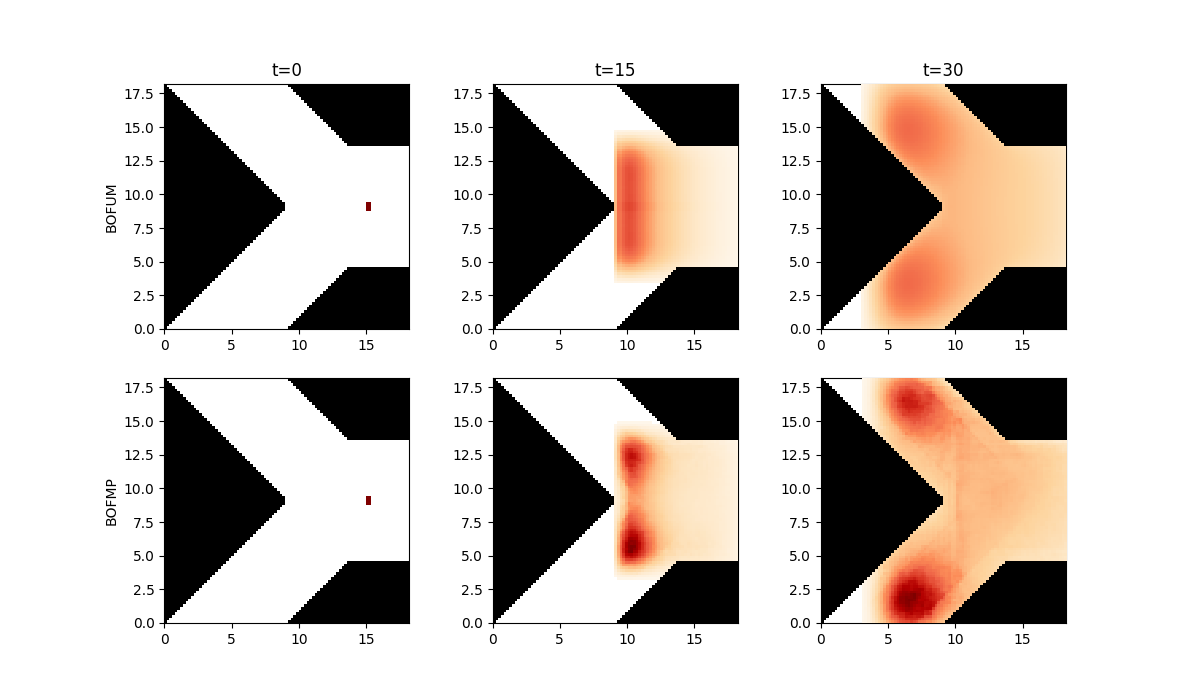
\includegraphics[width=\textwidth]{figures/idea.png}
    \caption{Occupancy predictions for BOFUM and our proposed BOFMP after several time steps. The map shows a T-section. At $t=0$, a person is shown as a red rectangle and with initial velocity towards left. At $t=15$, the person encounters intersection. BOFUM has no information about human motion pattern, and continues to propagate occupancy towards left. Our BOFMP knows that humans are likely to turn to either upper or lower corridors. At $t=30$, since occupancies going left vanish due to the wall, BOFUM predicts occupancies in corridors, but they are biased towards walls on the left. Our BOFMP predicts more occupancies in the middle of corridors, since it knows humans are more likely to walk in the middle.}
    \label{fig:idea}
\end{figure}

Human trajectories in indoor environment follow some motion patterns. For example, when there is corridor, humans tend to walk in the middle of the corridor, instead of walking besides the walls. To incoporate this human motion into tracking algorithm, we proposed \textit{Bayesian Occupancy Filte Using Motion Pattern}(BOFMP). The idea is shown in Figure \ref{fig:idea}.

The main contributions of this thesis work are summarized as following:

\begin{my_enumerate}
\item Neural Network Training.
\item Human Trajectory Simulation.
\item Object Tracking using Bayesian Occupancy Filter
\item Comparision between BOFUM and BOFMP
\end{my_enumerate}

\section{ Neural Network Training}  To capture  human motion patterns, we trained neural networks to learn how a walking person changes directions at different locations on a given map. Mathmatically, there are two ways to represent the motion pattern, either using conditional probability or joint probability. For the former one, given a grid map as input, the network learns for each given grid cell \( c \) on the map, the probabilities of next possible velocity \( V \) conditioned on last velocity \( V^- \):

\[ P_c\{V | V^-\} \] 

Alternatively, the network can also learn the joint probability:

\[ P_c\{V , V^-\} \]

Theoretically, it is always better to have joint probability, since conditional probability can be caculated from joint probability by marginalization and Baye's rule. However, due to reasons explained in Section \ref{section:hms}, we are not able to get accurate joint probabilities as ground truth. Therefore, the network is trained to learn \( P_c\{V | V^-\} \). 

\begin{figure}[ht]
  \centering
   \captionsetup{width=\linewidth}
    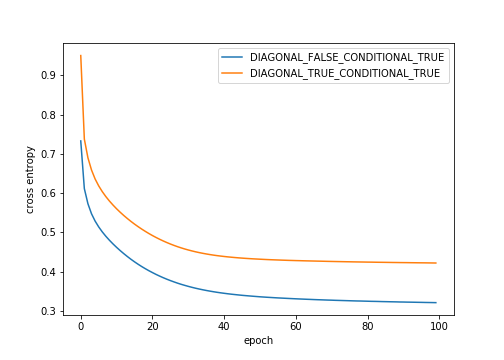
\includegraphics[width=.7\textwidth]{figures/trainning_history.png}
    \caption{Cross entropy loss for trainning networks. We trained networks to learn conditional probabilities \( P_c\{V | V^-\} \). The green line shows trainning dynamics using data generated with directions "left, right, up and down". The yellow line also takes diagonal directions into account, which has 8 directions in total. Naturally, since more directions implies higher complexity, the overall loss for yellow line is higher than green line.}
    \label{fig:trainning}
\end{figure}

The network consists of 31 convolutional layers. It has both down-sampling path for extracting high-level features and up-sampling path for recovering full resolution. The network is trained with mini-batches of size of 128, and  is optimized with Adam optimizer. The training runs for 100 epoches, with early stopping patience of 15 epoches. Figure \ref{fig:trainning} shows the cross entropy loss during training.

\section{Human Trajectory Simulation} \label{section:hms}

To acquire enough amount of data for trainning our netwrok is expensive, especially when we have to consider all possible motion changes for every cell in a grid map. For non-diagonal directions, there are \( 4\times4=16\) possible motion changes. For diagonal directions, it goes up to \( 8\times8=64\). To get statistically sound motion pattern probabilities, it requires to record human trajectories on many different maps over a long period of time. However, due to practical reasons, we are not able to get that much real data. Instead, we simulate human trajectories with A-star algorithm from 6 real world maps with a total free space area of ca. \( 6.6\times10^3 \, m^2 \). For each cell on the map, we try to sample 5 trajectories starting from that cell. With those trajectories, we can caculate motion pattern probabilities. Then we take random crops of size \( 32 \times 32 \) cells from the real world maps as network inputs, and their corresponding probabilities as outputs. 

%\begin{figure}
%    \centering
%    \begin{subfigure}[h]{0.48\textwidth}
%        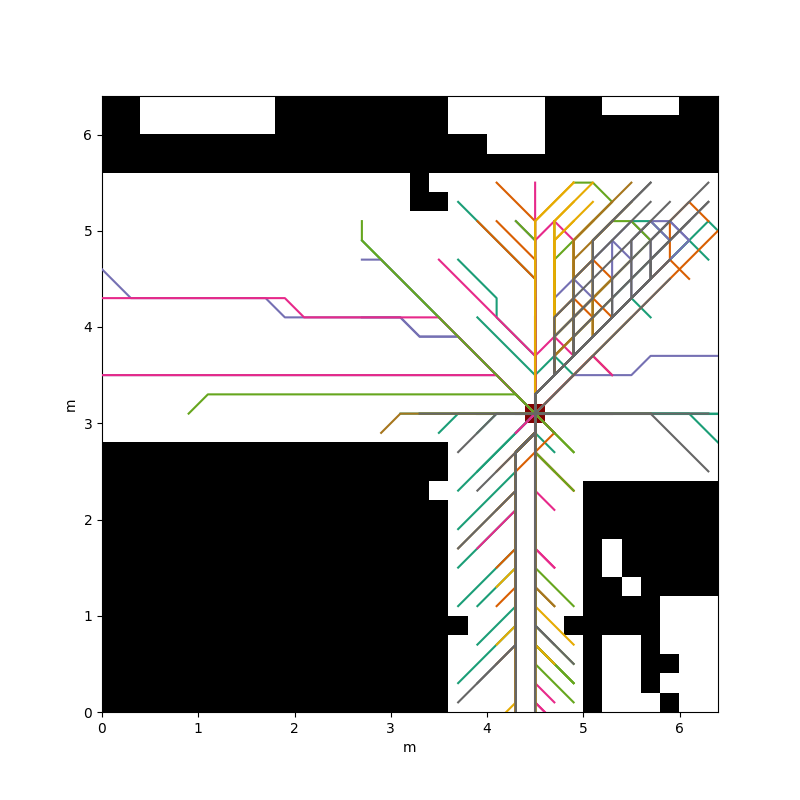
\includegraphics[width=\textwidth]{figures/trajs_through_cell.png}
%        \caption{A gull}
%        \label{fig:gull}
%    \end{subfigure}
%    ~ %add desired spacing between images, e. g. ~, \quad, \qquad, \hfill etc. 
%      %(or a blank line to force the subfigure onto a new line)
%    \begin{subfigure}[h]{0.48\textwidth}
%        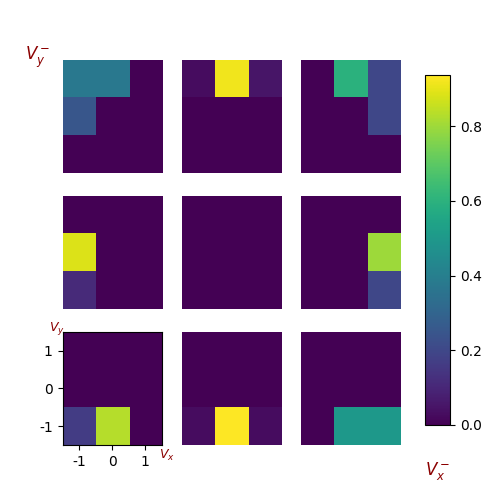
\includegraphics[width=\textwidth]{figures/probs_on_that_cell.png}
%        \caption{A tiger}
%        \label{fig:tiger}
%    \end{subfigure}
%
%    \caption{Pictures of animals}\label{fig:trajs}
%\end{figure}

\begin{figure}[h]
\begin{tabular}{ll}
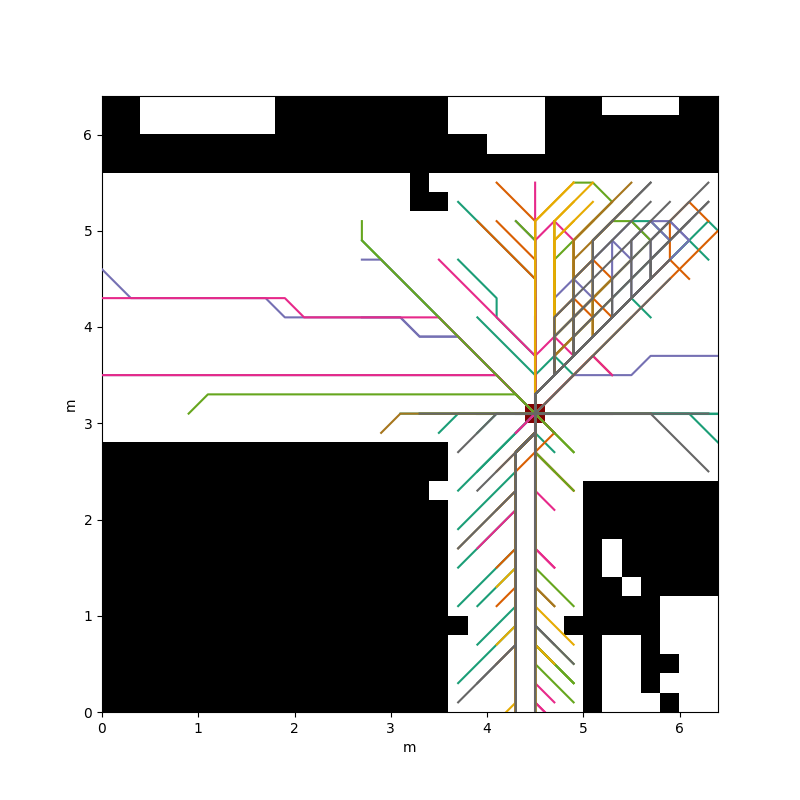
\includegraphics[width=0.48\textwidth]{figures/trajs_through_cell.png}
&
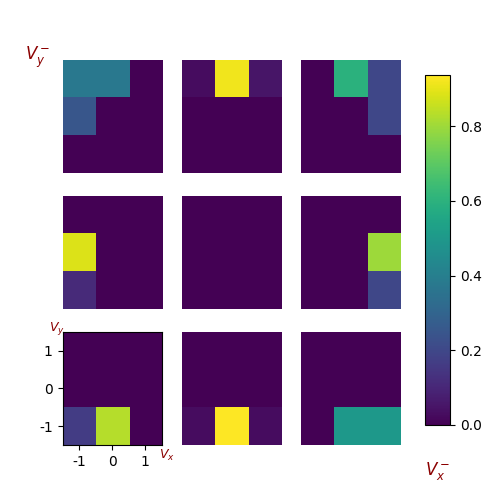
\includegraphics[width=0.48\textwidth]{figures/probs_on_that_cell.png}
\end{tabular}
\caption{\textbf{Left}: One example map crop as netwrok input. The map has size of \( 32 \times 32 \) cells, with resolution of \( 0.2m/cell\). It also shows trajectories that goes through the red cell. \textbf{Right}: Visualization of conditional probability \( P\{V | V^-\} \) for the red cell on left map. The axis shows velocities on \( x, y\) directions. Outter axes represent last velocity \( V^- \), and inner represent next velocity \( V \). One can see that \( P\{V=(-1, -1) | V^-=(-1, -1)\} = 0.21 \) and \( P\{V=(0, -1) | V^-=(-1, -1)\} = 0.79 \). This indicates that if a person reaches the red cell from upper right, it is very likely he will go downwards. }. 
\label{fig:trajs}
\end{figure}

Figure \ref{fig:trajs} shows one example of network input and the ground truth for one cell on the map. The number of samples we generated are summarized as follows:

\begin{center}
  \begin{tabular}{c|ccc}
    \hline
     & trainning & validation & test \\ \hline
    number of samples & 27,119 & 4,785 & 3,760\\
    \hline
  \end{tabular}
\end{center}

\section{Object Tracking using Bayesian Occupancy Filter}

Generally, Bayesian filter works in a recursive way and the filtering process can be decomposed into two stages: \textbf{prediction} and \textbf{correction}. For each time step, it firstly predicts the next state. After prediciton, when the new measurement is obtained, it corrects its prediction based on measurement. For Bayesian occupancy filter used in tracking applications, the state of world is represented by, for each cell on the grid map, the probabilities of cell's velocities and occupancy. However, the measurement gives information about only whether a cell is occupied or not at each time step. In order to make predicitions for the next time step, the filter has to infer velocities of each cell based on past occupancy information from measurements. Figure \ref{fig:correction} shows how BOFMP filter updates at one time step.


\begin{figure}[ht]
  \centering
   \captionsetup{width=\linewidth}
    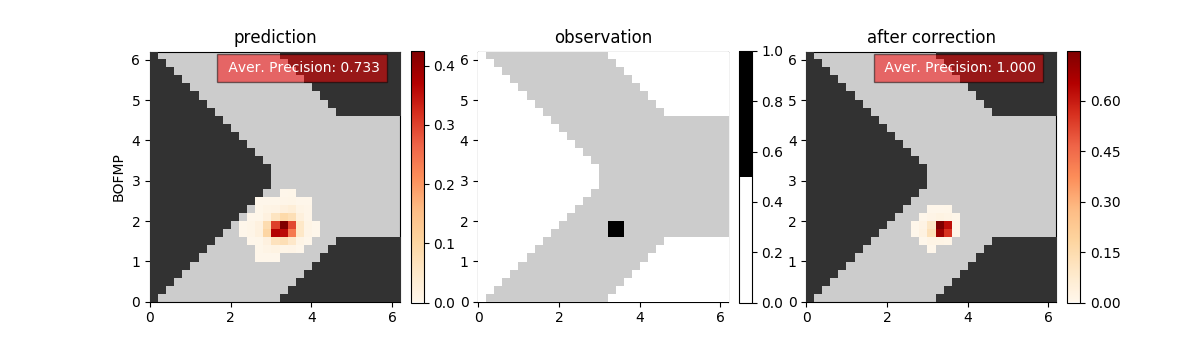
\includegraphics[width=\textwidth]{figures/correction_step.png}
    \caption{One filtering step of BOFMP filter. At last time step, the tracking object goes from up to down. Based on motion pattern, BOFMP predicts that there are possibilities that this object will trun to left-down and keep going downwards. After measurement shows that this obejct still goes downwards, BOFMP corrects its predictions and attenuates probabilities of turning left-down. Since the measurement adds additional information for BOFMP to make better predictions, the average precision increases after correction step.}
    \label{fig:correction}
\end{figure}

\section{Comparision between BOFUM and BOFMP}

To compare the performance of BOFUM and BOFMP, we consider two scenarios:

\begin{my_enumerate}
\item \textbf{tracking}. Measurements are given at each time step, and we evaluate consistency between occupancy predicton and the ground truth at every time step before a certain time point \( t \) .
\item \textbf{future prediction}. From time point \( t \) on, the measurement is no longer given. Then we evaluate occupancy predictions with ground truth for the next \( n \) time steps.
\end{my_enumerate}

The parameters of a BOF filter are:
\begin{my_enumerate}
\item \textbf{extent \( e\)}. It determines the maximum velocity of a cell. For example, if extent is 7, the velocities are in range  \( [-3, 3] \) cells/time step on both \( x \) and \( y \) axis. Since our neural network only models velocities within \( [-1, 1]\), we need firstly extend it to higher velocities. The details on how we do this will be explained in the thesis. 
\item \textbf{noise variance \( \delta^2\)}. Both BOFUM and BOFMP assume the tracking object has a constant velocity, with a Gaussian distributed acceleration noise. This parameter determines how likely an object accelerates or decelerate.
\item \textbf{omega \( \Omega \)}. In the correction step of BOF filters, measurments from sensors are incorporated into filter's prediction. Since sensor could be noisy, this parameter determines how much do we trust our measurements. The sensor used for our tracking application is laser rangefinder, which is rather physically reliable and therefore has a low \( \Omega \) value.
\end{my_enumerate}

The possible metrics that could be used for measuring the consistency between occupancy predicition and ground truth are: \textit{cross entropy}, \textit{f1 score} and \textit{average precision}.  We choose average precision as our metric and the reasons will be detailed in the thesis. To prove that our method is able to make predictions according to human motion pattern, we tune the parameters based on filter's performance for future predictions. For both filters, we randomly sample 100 sets of parameters from parameter ranges listed in Table \ref{table:param_range}, evaluate on tracking cases with time steps of 16 and caculate average precision for every time step over all tracking cases. Note that value range of noise variance $\delta^2$ for real data is higher than for simulated data. This is because in real data, there are higher uncertainties with human motion and sensor failures. The measurement is lost at time step \( t=9\), and we select the best set of parameters based on the average of average precisions for the next \( 8 \) time steps. 

\begin{table}[H]
\centering
  \begin{tabular}{c|c|c}
    \hline
     &   value range for simulated data & value range for real data \\ \hline
    \( e \) & \( \{3, 5, 7\} \) &  \( \{3, 5, 7\} \)\\
    \(  \delta^2\) & \( [0.1, 0.6]\) & \( [0.2, 0.7]\) \\   
   \( \Omega \) & \( [0.01, 0.2] \) & \( [0.01, 0.2] \)\\
   \hline
 \end{tabular}
\label{table:param_range}
\caption{Parameter ranges for BOF filters.}
\end{table}

\subsection{On simulated data}

We generated 500 tracking cases as validation set for tuning filter parameters and 500 tracking cases for test set. Validation and test cases are generated from different maps, and on each map, there are either one or two walking humans. We firstly tuned the parameters on validation set for BOFUM and BOFMP individually. Then we apply both filters with their best parameters on test set. The best set of parameters and its corresponding average precision from \( t=9 \) to \( t=16 \) on test data are listed in Table \ref{table:best_param_simulated}. Figure \ref{fig:simulated_test_data} shows mean of average precision over 500 test cases for each time step.

\begin{table}[H]
\centering  
\begin{tabularx}{\textwidth}{c|c|c|c|c|c}
    \hline
    & $ e $ & $ \delta^2 $ & $ \Omega $ & average precision for $t=8:16 $ & mean\\ \hline
    BOFUM & 7 & 0.556 & 0.0164 &  0.767  0.599  0.500    0.416  0.349  0.279  0.232  0.192 & 0.417 \\
    BOFMP & 7 & 0.373 & 0.0353 & 0.785  0.637  0.552  0.479  0.416  0.358  0.311  0.252 & 0.474 \\
   \hline
  \end{tabularx}
\label{table:best_param_simulated}
\caption{Best parameters for BOFUM and BOFMP on simulated data.}
\end{table}


\begin{figure}[ht]
  \centering
   \captionsetup{width=\linewidth}
    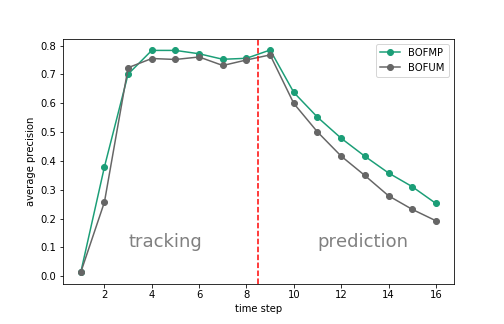
\includegraphics[width=.8\textwidth]{figures/test_on_simulated_data.png}
    \caption{Evaluation results on test data. The average precision for both filters start with values close to zero. Since we highly trust our measurments (low $\Omega$), both filters are able to successfully track the objects within 3 time steps. The fact that average precision keeps a high vaule from $t=3$ to $t=8$ indicates that both filters can predict very well for the next immediate time step. Starting from $t=9$ (see the red dash line), measurements are no longer given. The prediction is still accurate for the next time step ($t=9$), but decreases progressively over time.  This is expected, since without measurements, the state of world becomes more and more uncertain. Even though, we can see that our BOFMP have a higher average precision value than BOFUM at almost every time step, which indicates the improvements of our method in both tracking and future predicition stages.}
    \label{fig:simulated_test_data}
\end{figure}

Figure \ref{fig:tracking_simulated_data} shows how BOFUM and BOFMP perform tracking on one case from test data. In this example, a person is walking from the lower door towards upper door. The grey curve on the map shows the trajectory of the person. At $t=8$, the person walks with upwards velocity of 1 cell/time step. Both algorithms track the person very well with average precision of $1.0$. At $t=9$, the measurement is lost and future prediction stage of tracking starts. At $t=10$, BOFUM predicts that the person will still goes upwards, with a low possibility going other directions. However, since BOFMP knows there is a door above, it predicts that the person is also very likely going to that door, and therefore turns to upper left. At later time steps, BOFMP continues to predict occupancy probabilities towards upper door as well as other possible directions (i.e., door on the left and empty space on the right). On the contrary, BOFUM still propagates most occupancies upwards. At $t=16$, since the object accelerates to higher velocity, most of occupancy predictions of BOFMP are left behind the tracking object.
\begin{figure}[ht]
  \centering
   \captionsetup{width=\linewidth}
    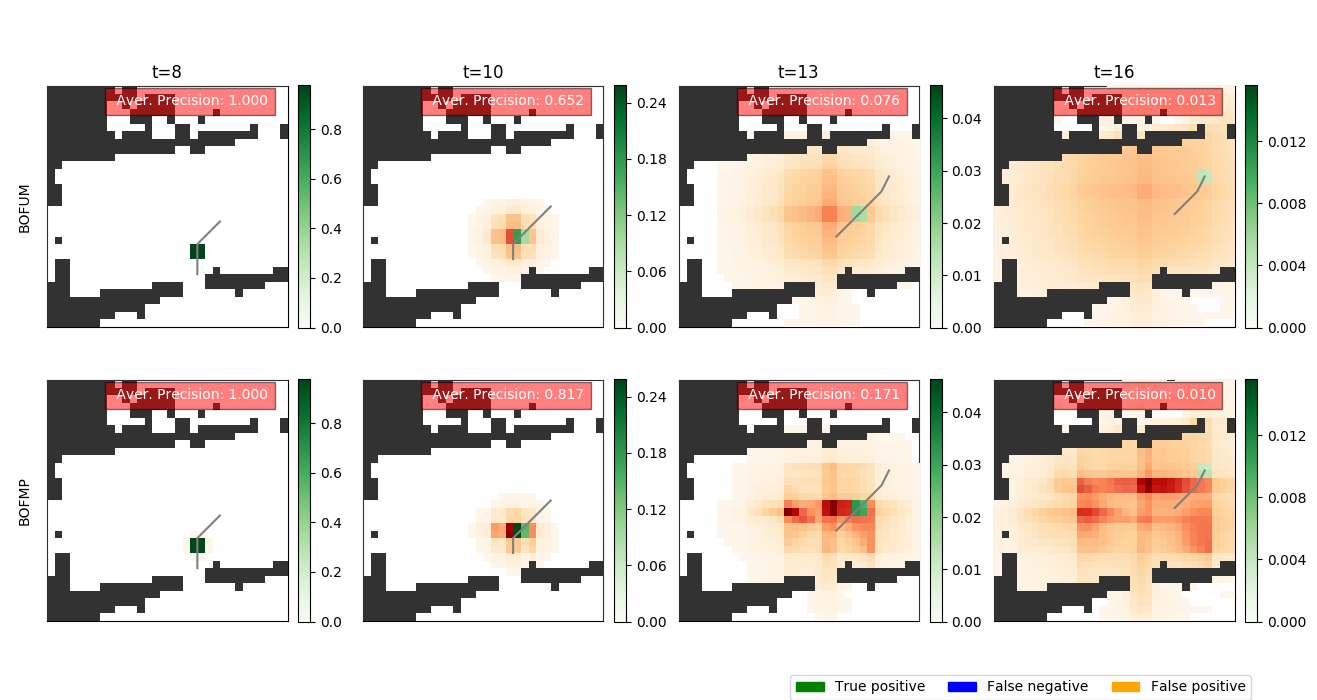
\includegraphics[width=\textwidth]{figures/tracking_sample_for_simulated_data.png}
    \caption{One example of tracking case from test data.}
    \label{fig:tracking_simulated_data}
\end{figure}

\subsection{On real data}

Although our neural network are trained on simulated human trajectories, we expect that our method also outperforms BOFUM on real tracking cases. We recorded human trajectories on two different ground plans by a laser rangefinder mounted on a robot. After processing raw laser data, we get 500 tracking cases for validation from one of the ground plans and 244 for test from the other. 



\textbf{Spatial blurring of motion probabilities}

The simulated trajectories do not always reflect real human's motion patterns. This is because, as shown in Figure \ref{fig:blur_idea}, humans are more flexible to decide when to make turns. 

\begin{figure}[ht]
  \centering
   \captionsetup{width=\linewidth}
    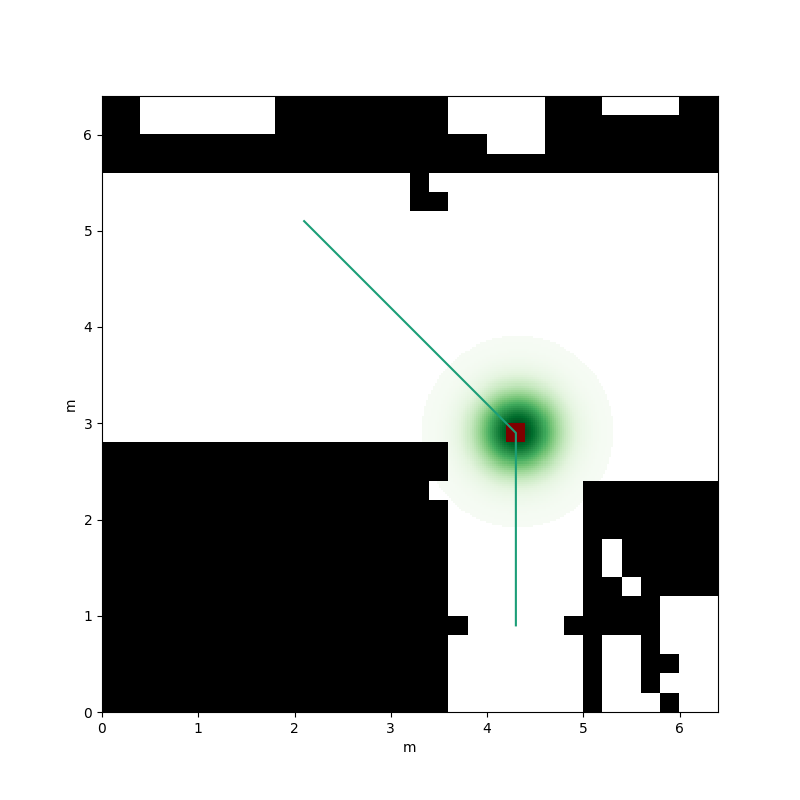
\includegraphics[width=.6\textwidth]{figures/blur_idea.png}
    \caption{A turn on simulated human trajectory. In order to reach the goal location in upper left corner, the simulated trajectory shows that a person will make a turn from going up to going up-left at location indicated by the red square. However, in real scenarios, a person is more flexible in deciding where to make that turn and he might turn at any location in the green area.}
    \label{fig:blur_idea}
\end{figure}

Therefore, to better adapt to real data, we introduce a techinique that blurs the motion probabilities  \( P_c\{V | V^-=v\} \) of a cell $c$ spatially into its neighbors if a \textit{turn} is detected. A \textit{turn} on cell $c$ for velocity $v^-$ is defined as:

\[ 
turn_c(v^-) = 
\begin{cases}
    True , & \text{if} \quad \argmax_v (P_c\{V=v | V^-=v^-\}) \, != \, v^- \\
    False,              & \text{otherwise}
\end{cases}
 \]


For each turn detected from motion pattern, we apply Gaussian blur spaitally to its neighbor cells' motion probability $P\{V | V^-=v^-\}$. As a consequence, another two parameters, blur extent \( blurExt \) and blur variance  \( blurVar \), are introduced and their value ranges are listed in Table \ref{table:spatial_blur_param_range}.


\begin{table}[H]
\centering  
\begin{tabularx}{.8\textwidth}{c|c|c}
    \hline
      &  \textit{value range } & \textit{note} \\ \hline
    \( blurExt \) & \( \{3, 5, 7, 9\} \) & \footnotesize{determines how far the Gaussian blur can reach} \\
     \( blurVar \) & \( [0.5, 2]\) & \footnotesize{ variance of the Gaussian kernel used for blurring} \\   
   \hline
  \end{tabularx}
\label{table:spatial_blur_param_range}
\caption{Parameters introduced by spatial blurring and their value ranges.}
\end{table}

\textbf{Motion keeping for future prediction}

Our proposed BOFMP, just like BOFUM, is \textit{memory-less}. That is to say, the last step of trakcing stage has absolute influence on future predictions, and the steps before the last step has no influence at all. In the real data we recorded, a time step equals to 0.25 second in real time. However, this short period of time is not able to summarize human's motion in the past time steps. Therefore, we propose to add moving average velocity of last few steps to the predicted velocity $P\{V_{pred}\}$, and then caculate next velocity $P\{ V \}$ from it. This process of incorporating moving average velocitiy is called as \textit{motion keeping}. It starts from the beginning of future prediction stage and the influence of moving average velocity is exponentially decreased over the following time steps.

Motion keeping also introduces new parameters. Assume the measurement is lost since time step $t_{lost}$, the new parameters are: 
\begin{my_enumerate}
\item \textbf{window size $w$}. It determines how many last time steps are considered when caculate moving average velocity .
\item \textbf{initial motion factor \( initMF\)}. This coefficent determines at the beginning of future predicition stage (i.e., $t=t_{lost}$), how much of moving average velocity $P\{V_{ma}\}$ is incorporated into predicted velocity $P\{V_{pred}\}$. 
\item \textbf{keep motion factor \( keepMF \)}. This constant is the base of the exponential function used to decrease moving average velocity $P\{V_{ma}\}$ over the following time steps. Therefore, for $t \geq t_{lost}$, 

\begin{align}
factor &= initMF \times keepMF^{(t-t_{lost})} \\
P\{V_{merge}\} &= factor \times P\{V_{ma}\} + (1-factor) \times P\{V_{pred}\}
\end{align}

\end{my_enumerate}

The value ranges of these parameters are listed in Table \ref{table:motion_keeping_param_range}. One example of tracking on real data using motion keeping is shown in Figure \ref{fig:keep_motion_idea}.
\begin{table}[H]
\centering  
\begin{tabularx}{.3\textwidth}{c|c}
    \hline
      &  \textit{value range } \\ \hline
    $w$ & \( \{2, 4, 6\} \)  \\
     $initMF$ & \( [0.3, 0.8]\) \\  
     $keepMF$ & \( [0.3, 0.8]\) \\    
   \hline
  \end{tabularx}
\label{table:motion_keeping_param_range}
\caption{Parameters introduced by motion keeping and their value ranges.}
\end{table}

\begin{figure}[ht]
\centering
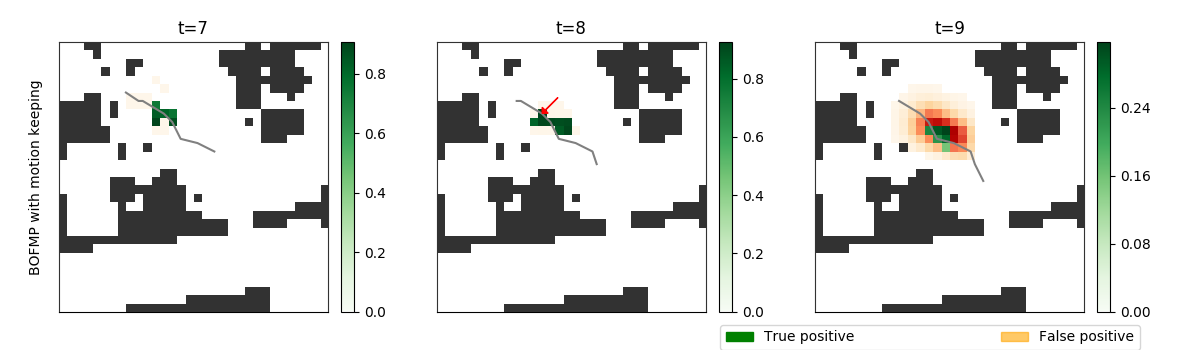
\includegraphics[width=\textwidth]{figures/moving_average_tracking.png}
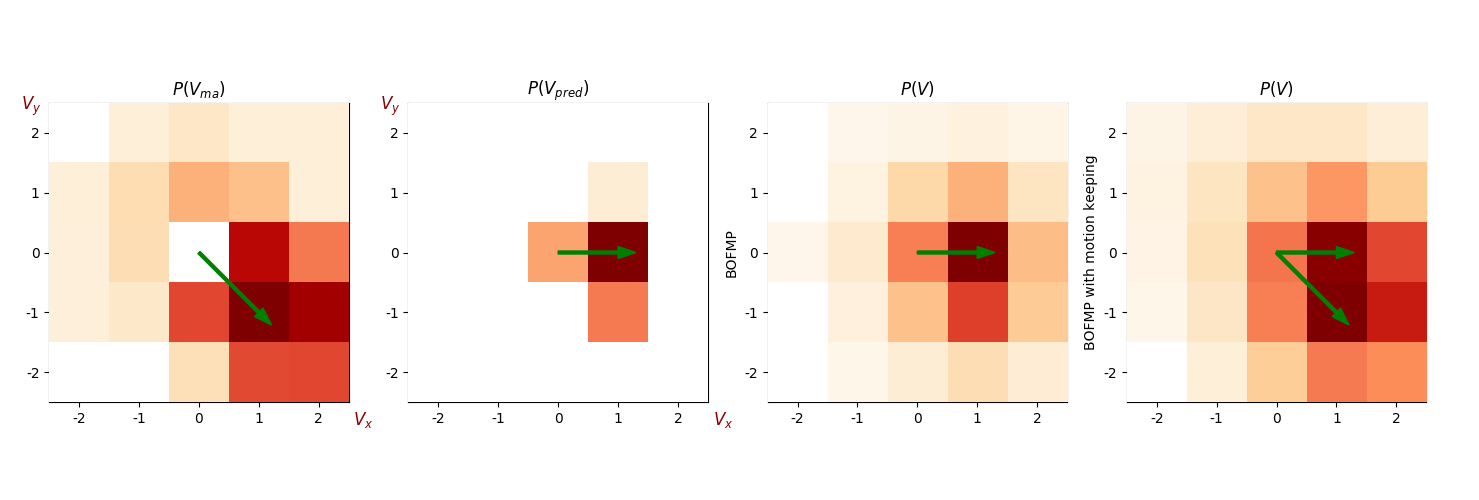
\includegraphics[width=\textwidth]{figures/moving_average_tracking_velocities_1.png}
\caption{\textbf{Up}: Three tracking steps of BOFMP with motion keeping. A person is walking from upper left towards lower right. The measurement is lost at $t=9$. \textbf{Down}: Velocities of the cell pointed by the red arrow at $t=8$. On each plot, the most possible direction is shown by the green arrows. Based on measurements from $t=7$ and $t=8$, the predicted velocity $P\{V_{pred}\}$ shows it is more likely the occupancy will propagates towards right for the next time step. However, past motion trend, which is represented by $P\{V_{ma}\}$, shows it is more likely to move to lower right. As a consequnce, BOFMP with motion keeping shows there are possibilities going both right and lower right, which is more realistic in this tracking example.}
\label{fig:keep_motion_idea}
\end{figure}


We randonly sample 100 sets of parameters for each scenario, evaluate them on validation set, and select the best set of parameters based on the mean of average precisions for the future prediction stage ($t=9:16$). The best parameters are shown in Table \ref{table:best_param_real}.

\begin{table}[H]
\footnotesize
\centering  
\begin{tabularx}{\textwidth}{c|c|c|c|c|c|c|c|c|c}
    \hline
    & $ e $ & $ \delta^2 $ & $ \Omega $ & \sml{blurExt} & \sml{blurVar} & $w$ & \sml{initMF} & \sml{keepMF}  & \footnotesize{mean a.p.}\\ \hline \hline
    BOFUM & 5 & 0.677 & 0.152  & - & - & - & - & - & 0.302   \\ \hline
    BOFMP & 5 & 0.649 & 0.191  & - & - & - & - & - & 0.321  \\
    \scriptsize{BOFMP spatial blurring} & 5 & 0.636 & 0.100  & 5 & 1.093 & - & - & - & 0.327  \\
    \scriptsize{BOFMP motion keeping} & 7 & 0.744 & 0.026  & - & - & 4 & 0.563 & 0.707 & 0.381  \\
   \hline
  \end{tabularx}
\label{table:best_param_real}
\caption{Best parameters for BOFUM and BOFMP on real data.}
\end{table}

\normalsize
Then we apply each filter with its best parameters on test data of 244 tracking cases. Figure \ref{fig:real_test_data} shows the average precision for each time step, and Table \ref{table:real_test_data} lists the average precision in future prediction stage and their mean. Compared with BOFUM, our methods have performance gain of $29\%$, $31\%$ and $43\%$ respectively.

\begin{table}[H]
\footnotesize
\centering  
\begin{tabularx}{.8\textwidth}{c|c|c}
    \hline
    & average precision for $t=9:16$ & mean \\ \hline \hline
    BOFUM & 0.670   0.512  0.384  0.314  0.252  0.205  0.167  0.148  & 0.331   \\ \hline
    BOFMP & 0.705  0.570   0.468  0.424  0.351  0.336  0.305  0.255 & 0.427  \\
    \scriptsize{BOFMP spatial blurring} & 0.694  0.564  0.480   0.439  0.371  0.349  0.311  0.264 &  0.434  \\
    \scriptsize{BOFMP motion keeping} &  0.762  0.675  0.561  0.496  0.405  0.353  0.305  0.238 & 0.474  \\
   \hline
  \end{tabularx}
\label{table:real_test_data}
\caption{Future predictions for BOFUM and BOFMP on real data.}
\end{table}
\normalsize

\begin{figure}[ht]
  \centering
   \captionsetup{width=\linewidth}
    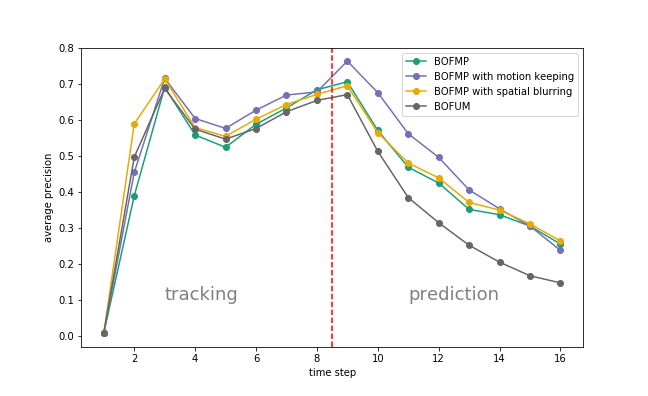
\includegraphics[width=.8\textwidth]{figures/test_on_real_data.png}
    \caption{Evaluation results on real test data. Like for simulated data, average precision starts with values close to zero, and increase rapidly over the next two time steps. From $t=3$ to $t=8$, average precisions keep rather stable at high values, which proves that filters predict very well for the next immediate step. In future prediction stage ($t=9:16$), average precisions decrease severely as time horizon increases, since the state of the world becomes more uncertain. However, our BOFMP and its variations are still better than BOFUM for every time step in this stage.}
    \label{fig:real_test_data}
\end{figure}

To conclude, we proposed a Bayesian occupancy filter that utilizes human motion pattern for tacking humans in indoor environments. The motion patterns are gained from a neural network which is trained on simulated human trajectories. Our proposed method outputforms BOFUM on both simulated and real tracking cases. One of the most important advantages of our method is that, although the motion pattern is derived from simulated data, it is applicable on real tracking scenarios.  












%############# appendix #################
\cleardoublepage
\renewcommand{\chaptername}{\appendixname} %if name appears in header

% \begin{appendix}

% \chapter{Keyword Lists and Topic Names} \label{appendix2}
\setlength{\LTleft}{-20cm plus -1fill}
\setlength{\LTright}{\LTleft}
\begin{longtable}[c]{| p{.10\linewidth} | p{.60\linewidth} | p{.30\linewidth} |} 
    \hline
     & \textbf{Keywords} & \textbf{Topic name} \\
    \hline
    \hline
    1 &  bone lupron scan chemo months casodex hormone mets treatment started adt side scans effects trial radiation therapy oncologist drug shot & therapies and treatments \\
    \hline
    2 &  post thread edited gmt forum moderator healingwell link members information posted email posts posting site click journey community member threads & general forum management \\
    \hline
    3 &  doctor told back good time asked week call appointment today didn't husband results called he's doc office weeks thought wanted & appointments with doctors \\
    \hline
    4 &  pca treatment make men time medical patient life case people read years doctors information find good point patients things diseas & medical records  \\
    \hline
    5 &  surgery surgeon robotic gleason hospital open  good experience urologist diagnosed prostatectomy procedure post davinci age positive read vinci surgeons radiation  & surgery and surgery experience \\
    \hline
    6 &  months test month results year back years good post time surgery undetectable today radiation srt ago weeks level week blood & recall of experience with disease \\
    \hline
    7 &  pain back time day surgery days home night blood bladder hours catheter hospital morning side left week area weeks started & pain and blood-bladder issues \\
    \hline
    8 &  chat gfmph guys night home meet time trip join fun log room event meeting members plan awareness jeff word info & chat and trip \\
    \hline
    9 &  biopsy urologist years test gleason ago results dre age back doctor year months mri diagnosed found  scan blood negative normal & biopsy and MRI \\
    \hline
    10 &  rection viagra trimix surgery cialis sex pump injections erections months penis units injection good time dose sexual work side pills & erection and sex issue \\
    \hline
    11 &  room man car put water bag minutes home make virtue machine sling device made light hand wear house sitting guy & discussion on broad topics \\
    \hline
    12 &  url metformin radiation www research rad rel target kumc blank htm nucmed nofollow avodart marina failure doctor del rey lam & researches on radiation and medication \\
    \hline
    13 &  radiation treatment therapy side effects treatments imrt proton brachytherapy seeds hormone beam surger oncologist salvage brachy external hdr options months & side effects of radiation and other treatments \\
    \hline
    14 &  day surgery weeks catheter bladder incontinence days pads urine pad time night week dry months back post pee times remove & urine issues \\
    \hline
    15 &  www http usa article org news html link health interesting pca video watch htm net youtube site story articles thought  & news and articles from outside links \\
    \hline
    16 &  cells diet system immune exercise body cell supplements vitamin taking heart blood health eat weight healthy testosterone food found research & diet and exercise \\
    \hline
    17 &  insurance cost company drug pay medicare drugs approved health costs provenge cover year money plan fda order generic medical expensive  & insurance and payments \\
    \hline
    18 &  gleason lymph positive tumor report left pathology biopsy margins nodes invasion negative seminal tissue score margin cores grade surgery apex  & diagnosis \\
    \hline
    19 &  men patients study risk disease treatment clinical years survival screening trial therapy results percent group data studies early trials article & studies and clical trails \\
    \hline
    20 &  time good life years day year back feel hope great wife today people guys support love family friends things work & appreciations for life and families \\
    \hline
\caption{Topic keywords produced by \textit{MALLET} and the topic names.}
\end{longtable}

% %\cleardoublepage
% %!TEX root = thesis.tex
\chapter{Predefined Keyword List} \label{appendix3}
\vspace{-10pt}
\begin{table}[h]
\centering
\resizebox{.85\textwidth}{!}{
{\renewcommand{\arraystretch}{1}
   \begin{tabular}{| c | c | c | }
    \hline
     & \textbf {Keywords} & \textbf{Category} \\
    \hline
    \hline
    1 & \specialcell{Androgenentzugstherapie/Androgenentzug/ \\ Dreifache Hormonblockade/DHB} & \multirow{7}{*}{Therapy} \\ \cline{1-2}
    2 & \specialcell{Hormonentzug/Hormonablation/\\Antihormontherapie /AHT}  &  \\ \cline{1-2}
    3 & Androgendeprivationstherapie/ADT &  \\ \cline{1-2}
    4 & Robert Leibowitz MD/Robert Leibowitz & \\ \cline{1-2}
    5 & LHRH/LH-RH/GnRH/Gn-RH  & \\ \cline{1-2}
    6 & Antagonist  & \\ \cline{1-2}
    7 & Analoga & \\
    \hline
	8 & Bicalutamid/Casodex & \multirow{9}{*}{Drug} \\ \cline{1-2}
    9 & Abiraterone/Zytiga & \\ \cline{1-2}
    10 & Flutamid & \\ \cline{1-2}
    11 & Enzalutamid/Xtandi & \\ \cline{1-2}
    12 & Degarelix & \\ \cline{1-2}
    13 & Leuprorelin & \\ \cline{1-2}
    14 & Pamorelin & \\ \cline{1-2}
    15 & Buserelin & \\ \cline{1-2}
    16 & Lupron/Eligard & \\ \cline{1-2}
    \hline
    17 & Kastrationsniveau & \multirow{7}{*}{Effect} \\ \cline{1-2}
    18 & Kastration & \\ \cline{1-2}
	19 & Hitze & \\ \cline{1-2}
    20 & Hitzewallung & \\ \cline{1-2}
    21 & M\"digkeit/schlapp/m\"ude & \\ \cline{1-2}
    22 & Diabetes & \\ \cline{1-2}
    23 & Osteoporose & \\ \cline{1-2}
    \hline
    \end{tabular}
}
}
\caption{Predefined German keyword list for sentiment query.}
\end{table}

\newpage
%\vspace{50pt}
\begin{table}[p]
\centering
\resizebox{.85\textwidth}{!}{
{\renewcommand{\arraystretch}{1}
   \begin{tabular}{| c | c | c |}
    \hline
     & \textbf {Keywords} & \textbf{Category} \\
    \hline
    \hline
    1 & \specialcell{Total androgen blockage/TAB \\ /Triple Hormone blockade/blockage / \\ Triple androgen blocker }& \multirow{8}{*}{Therapy} \\ \cline{1-2}
    2 & \specialcell{Hormone therapy/treatment/blockage/HT}  &  \\ \cline{1-2}
    3 & Androgen deprivation therapy/ADT &  \\ \cline{1-2}
    4 & Robert Leibowitz MD/Robert Leibowitz & \\ \cline{1-2}
    5 & LHRH/LH-RH/GnRH/Gn-RH  & \\ \cline{1-2}
    6 & Antagonist  & \\ \cline{1-2}
    7 & Anti androgen/Anti-androgen  & \\ \cline{1-2}
    8 & Agonist & \\
    \hline
    9 & Lupron/Eligard & \\ \cline{1-2}
	10 & Bicalutamid/Casodex & \multirow{5}{*}{Drug} \\ \cline{1-2}
    11 & Abraxane & \\ \cline{1-2}
    12 & Cyclofosfamide & \\ \cline{1-2}
    13 & Enzalutamide/Xtandi & \\ \cline{1-2}
    14 & Degarelix & \\ \cline{1-2}
    \hline
    15 & Castrate level & \multirow{7}{*}{Effect} \\ \cline{1-2}
    16 & Castration & \\ \cline{1-2}
	17 & Heat & \\ \cline{1-2}
    18 & Hot flash & \\ \cline{1-2}
    19 & Fatigue & \\ \cline{1-2}
    20 & Diabetes & \\ \cline{1-2}
    21 & Osteoporosis & \\ \cline{1-2}
    \hline
    \end{tabular}
}
}
\caption{Predefined English keyword list for sentiment query.}
\end{table}


% \include{anhang3}
% \end{appendix}

% \cleardoublepage
% \phantomsection
% \addcontentsline{toc}{chapter}{\protect\numberline{List of Abbreviations}}
% %!TEX root = project_report.tex
\chapter*{List of Abbreviations}
\label{sec:abbreviations}
\markboth{\MakeUppercase{List of Abbreviations}}{\MakeUppercase{List of Abbreviations}} 
\begin{longtable}[t]{ll}
\arrayrulecolor{hsugrau}
\textbf{\textcolor{hsurot}{A}} &\\ \hline 
ANT & Allgemeine Nachrichtentechnik (Signal Processing and Communication)\\

  &\\ \textbf{\textcolor{hsurot}{C}} &\\  \hline 
 CNN & Convolutional Neural Network \\
 
   &\\ \textbf{\textcolor{hsurot}{E}} &\\  \hline 
 E-SVM & Exemplar-Support Vector Machine\\
 
    &\\ \textbf{\textcolor{hsurot}{G}} &\\  \hline 
 GUI & Graphical User Interface\\

  &\\ \textbf{\textcolor{hsurot}{H}} &\\  \hline 
HSU-HH & Helmut-Schmidt-University/University of the Federal Armed Forces Hamburg\\
HoG & Histogram of Gradients \\

  &\\ \textbf{\textcolor{hsurot}{I}} &\\  \hline 
ILSVRC & ImageNet Large Scale Visual Recognition Challenge\\

&\\ \textbf{\textcolor{hsurot}{M}} &\\  \hline 
MIT & Massachusetts Institute of Technology\\

&\\ \textbf{\textcolor{hsurot}{S}} &\\  \hline 
SVM & Support Vector Machine\\
SIFT & Scale-Invariant Feature Transform
\end{longtable}

%Softwareverzeichnis
% \cleardoublepage
% \phantomsection
% \addcontentsline{toc}{chapter}{\protect\numberline{List of Software}}
% \chapter*{List of Software}
\markboth{\MakeUppercase{List of Software}}{\MakeUppercase{List of Software}} 
\label{sec:software}
\begin{table}[htb]
	\centering
		\begin{tabular}{|l|l||l|l|}
		\hline
			\bfseries{Name} & \bfseries{Version} & \bfseries{URL} & \bfseries{Comment}\\
		\hline
		\hline
			MATLAB & R2015b & https://de.mathworks.com/ & MathsWorks\\
		\hline

		\hline
		\end{tabular}
	\caption{Used software.}
	\label{tab:VerwendeteSoftware}
\end{table}



% \cleardoublepage
% %########### Bibliography ##############
\clearpage % to get correct page no. in TOC
\phantomsection
\addcontentsline{toc}{chapter}{\protect\numberline{\bibname}}

\renewcommand{\chaptername}{} %if name appears in header

\renewcommand{\baselinestretch}{1}
\normalsize

% if enabling this command all references of the bib file are listed
% otherwise only the referenced books are listed in Bibliography section
%\nocite{*} 

%\bibliographystyle{unsrt}
%\bibliographystyle{alpha}
%\bibliographystyle{ALPHADIN}

%\bibliographystyle{IEEEtran} %IEEE Style
\bibliographystyle{plainnat}
	
% In literatur.bib sind die eigentlichen Literaturangaben enthalten
\bibliography{literatur} % requires file literatur.bib


\ifmakeindex
\cleardoublepage
\phantomsection
\addcontentsline{toc}{chapter}{\protect\numberline{Index}}
% Stichwortverzeichnis endgueltig anzeigen
\printindex
\fi

\end{document}
